\apendice{Manual de Kibana}

\section{Introducción}
Este anexo en un TFG convencional recibiría el nombre de \textit{Manual de usuario}, pero al consistir este TFG de un estudio, se ha decidido modificarlo a \textit{Manual de Kibana}, y se indagará en todas las posibilidades y caracterísiticas avanzas que ofrece el programa más visual e intuitivo de los tres componentes del stack ELK. 

\section{Requisitos de usuarios}
Este \textit{software} no requiere de gran cantidad de requisitos ni es muy demandante en recursos, puesto que trabaja sobre los datos procesados y optimizados previamente.
Para su uso se requieren los siguientes requisitos:
\begin{itemize}
    \item Acceso a Internet
    \item Acceso a un navegador convencional como pueden ser Google Chrome, Microsoft Edge o Brave entre otros.
    \item Acceso a un stack ELK.
    \item Que el sistema disponga de espacio un espacio de procesamiento suficiente para cargar y analizar las visualizaciones de datos.
    \item Habilidad para comprender visualizaciones de datos.
\end{itemize}

\section{Instalación}
El programa dispone de un \href{https://www.elastic.co/es/kibana}{sitio web oficial} donde su descarga e instalación es sencilla e intuitiva. También se incluyen guías y videotutoriales en caso de complicaciones en la instalación o ejecución.

\section{Manual del usuario}

Este software de visualización de datos, una vez sea descargado de su \href{https://www.elastic.co/es/kibana}{página oficial}, se tendrá que ejecutar el fichero \textit{kibana.bat} en el directorio \textit{bin} como se muestra en la ilustración \ref{fig:kibana1}. 

\begin{figure}
    \centering
    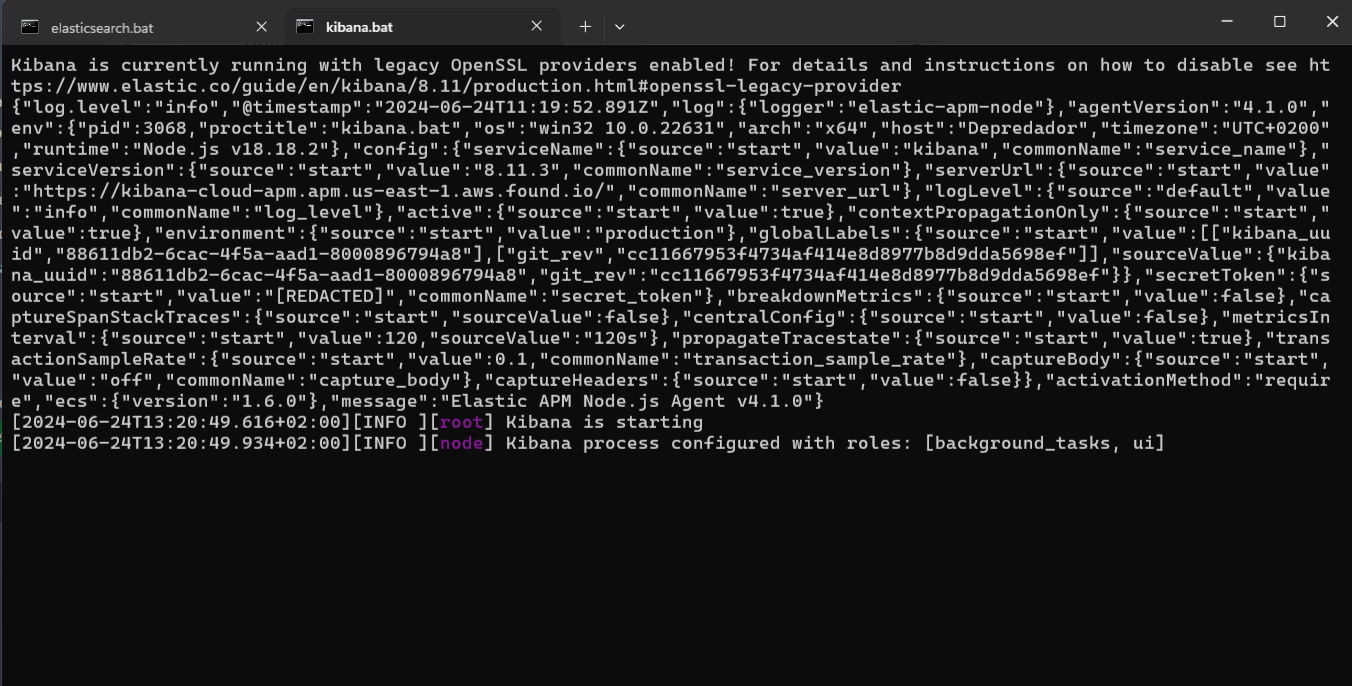
\includegraphics[width=1\linewidth]{img/kibanaa1.png}
    \caption{Visualización de terminal una vez se ejecute kibana.bat}
    \label{fig:kibana1}
\end{figure}

Pasados unos segundos, la terminal indicará que el servicio de Kibana está activo y para acceder a el nos iremos al navegador y nos dirigemos al puerto local 5601, en el cual se nos mostrará la interfaz gráfica de Kibana (ver ilustración  \ref{fig:kibana2}).

\begin{figure}
    \centering
    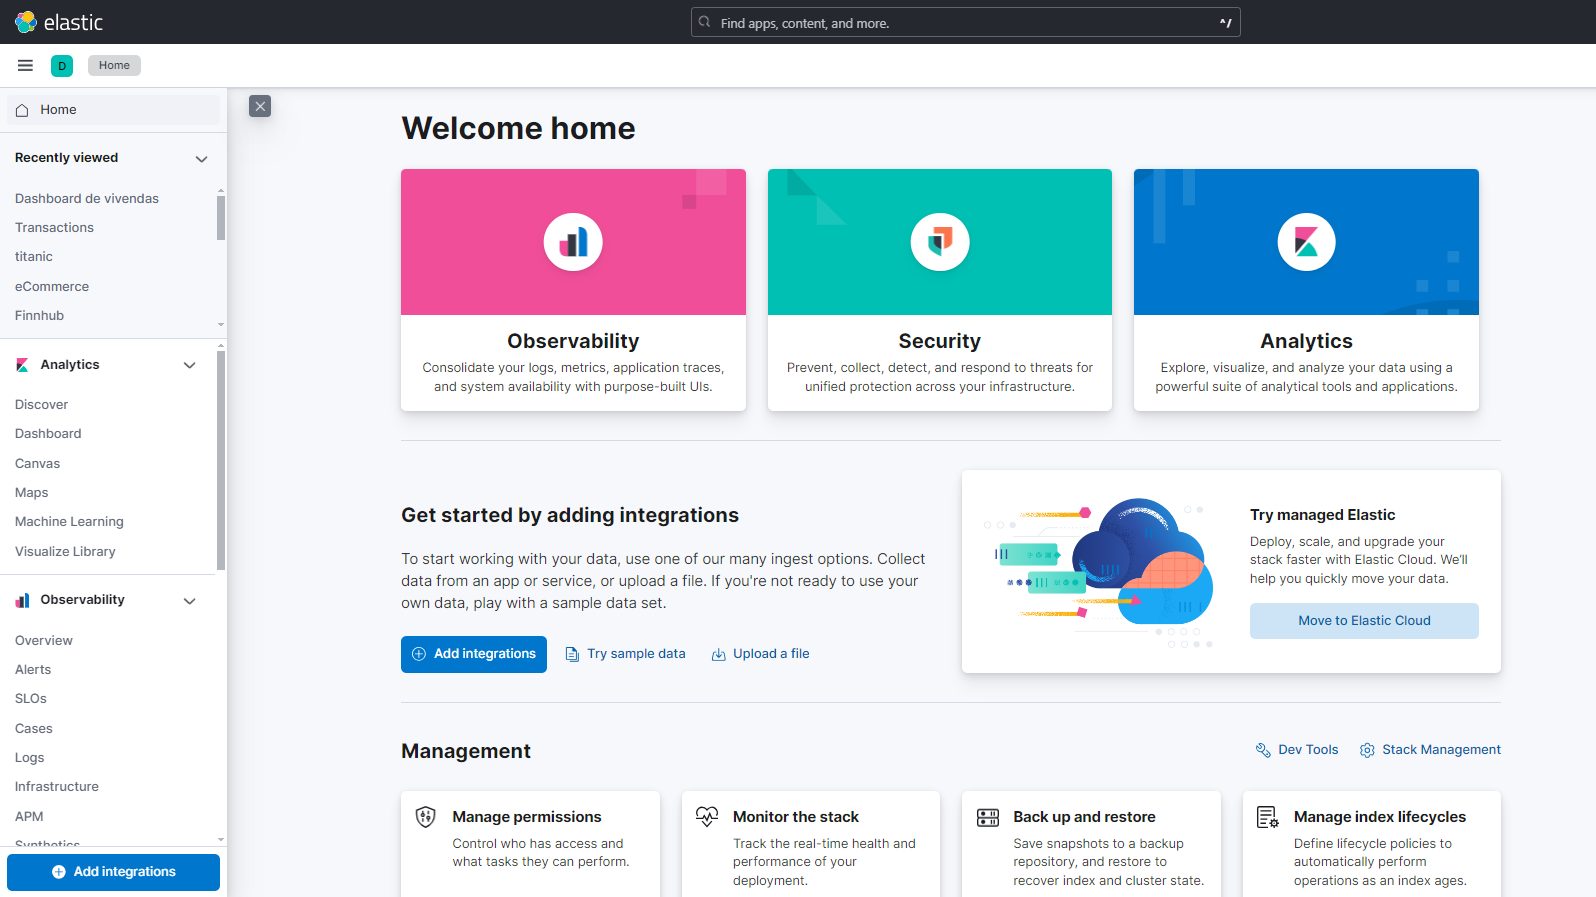
\includegraphics[width=1\linewidth]{img/kibana2.png}
    \caption{Interfaz gráfica inicial de Kibana.}
    \label{fig:kibana2}
\end{figure}

\paragraph{}
\paragraph{}
\paragraph{}
\paragraph{}


Una vez se llega a esta pantalla, se pueden observar las diferentes funcionalidades que ofrece Kibana. La primera en la que se va a indagar, y que es importante de cara a comprobar que los datos de los índices de ElasticSearch son los deseados, es la funcionalidad \textit{Analytics} (ver ilustración \ref{fig:kibana3}). La parte que más interesa es la de \textit{Discover}, en la cuál se van a mostrar todos los registros presentes en el índice que se indique. En este ejemplo se van a visualizar los datos del índice \textit{titanic} (ver ilustración \ref{fig:kibana4}), como se puede observar en la columna de la izquierda se muestran los campos disponibles junto al tipo al que pertenecen, pudiendo realizar filtrados personalizados pero no modificaciones. En la sección principal llamada \textit{Documents}, se muestran en detalle todos los datos de los registros presentes en el índice, permitiendo indagar más profundamente por si interesa alguno en concreto (ver ilustración \ref{fig:kibana6}).

\begin{figure}
    \centering
    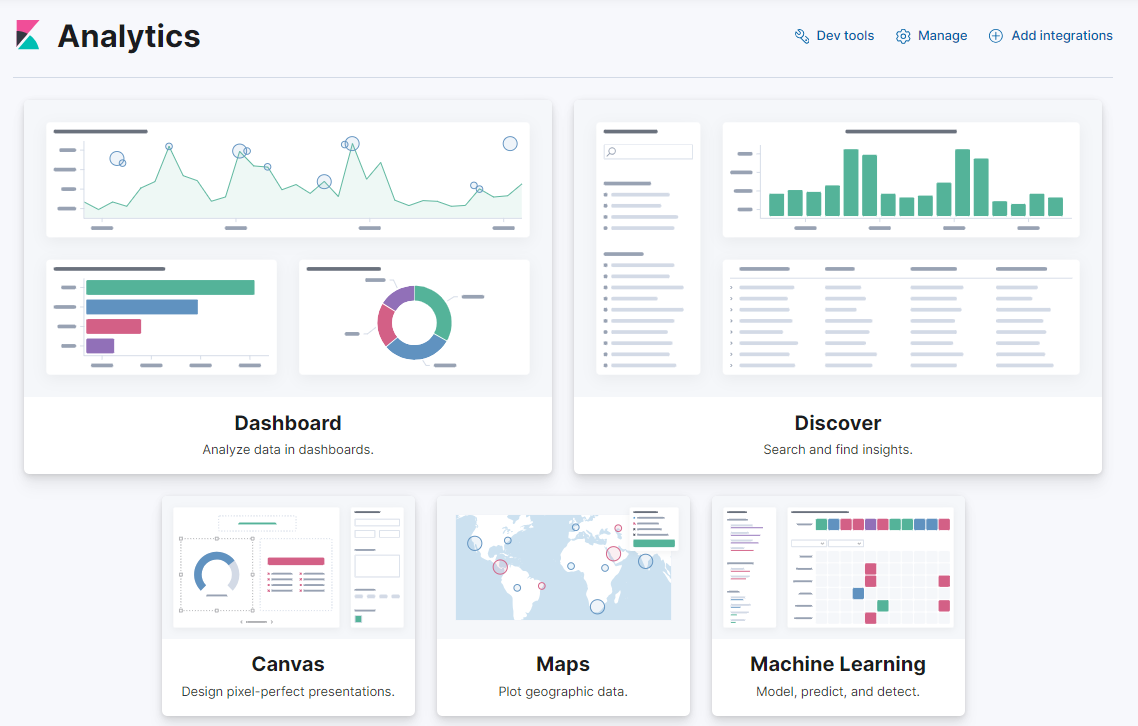
\includegraphics[width=1\linewidth]{img/kibana3.png}
    \caption{Visión general de la funcionalidad \textit{Analytics.}}
    \label{fig:kibana3}
\end{figure}

\begin{figure}
    \centering
    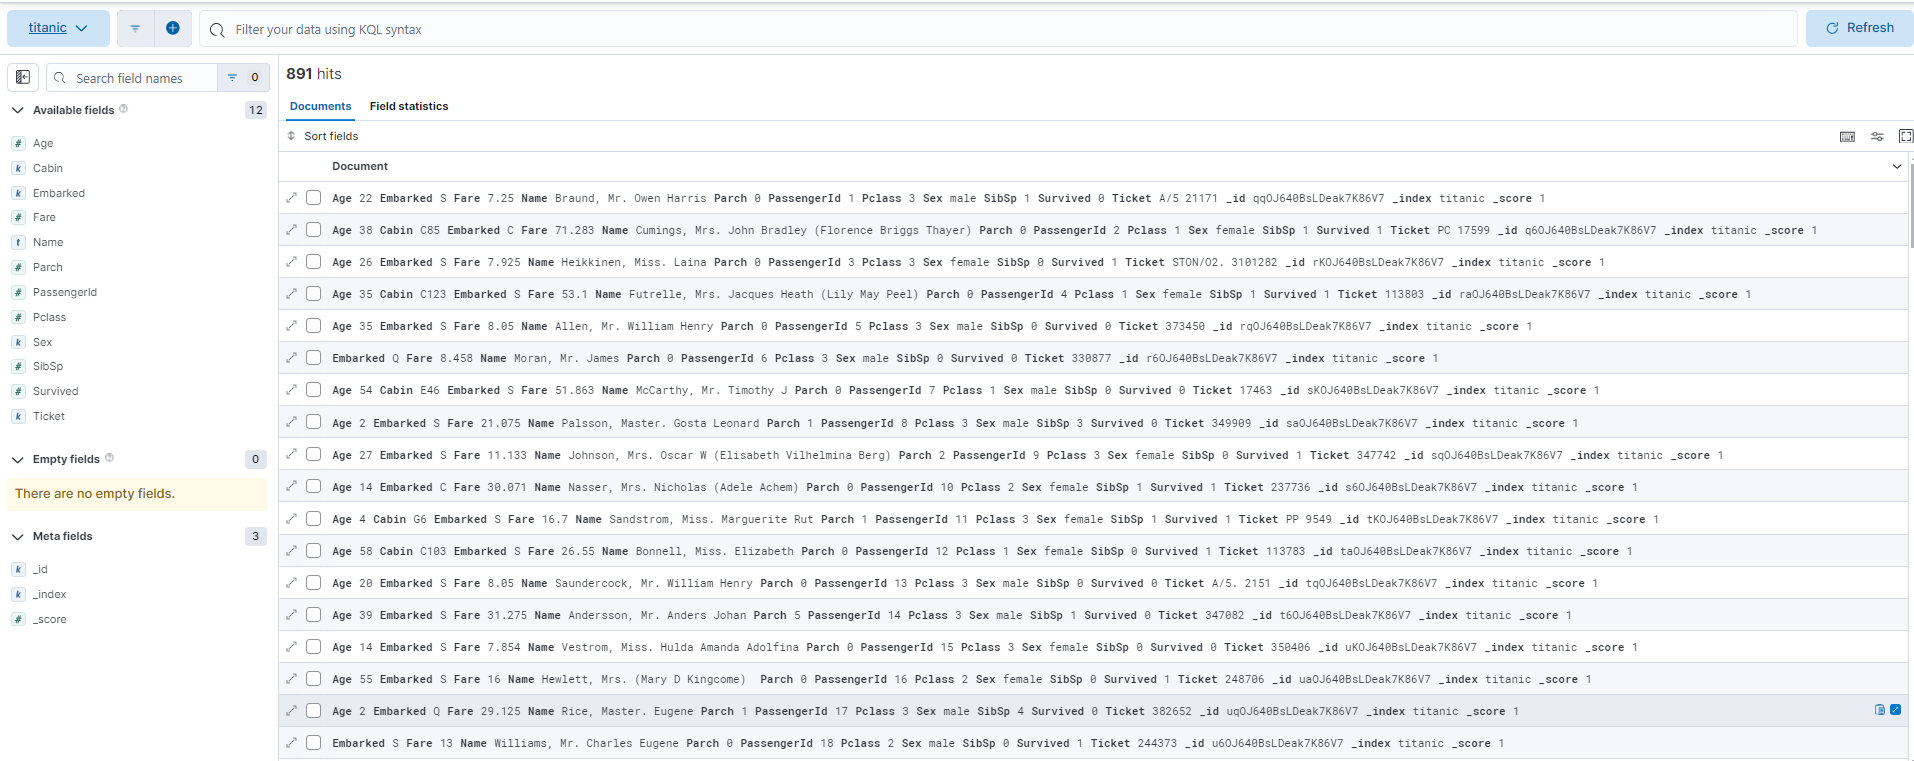
\includegraphics[width=1\linewidth]{img/kibana4.png}
    \caption{Visualización del \textit{Discover} de los datos del índice \textit{titanic}.}
    \label{fig:kibana4}
\end{figure}

\begin{figure}
    \centering
    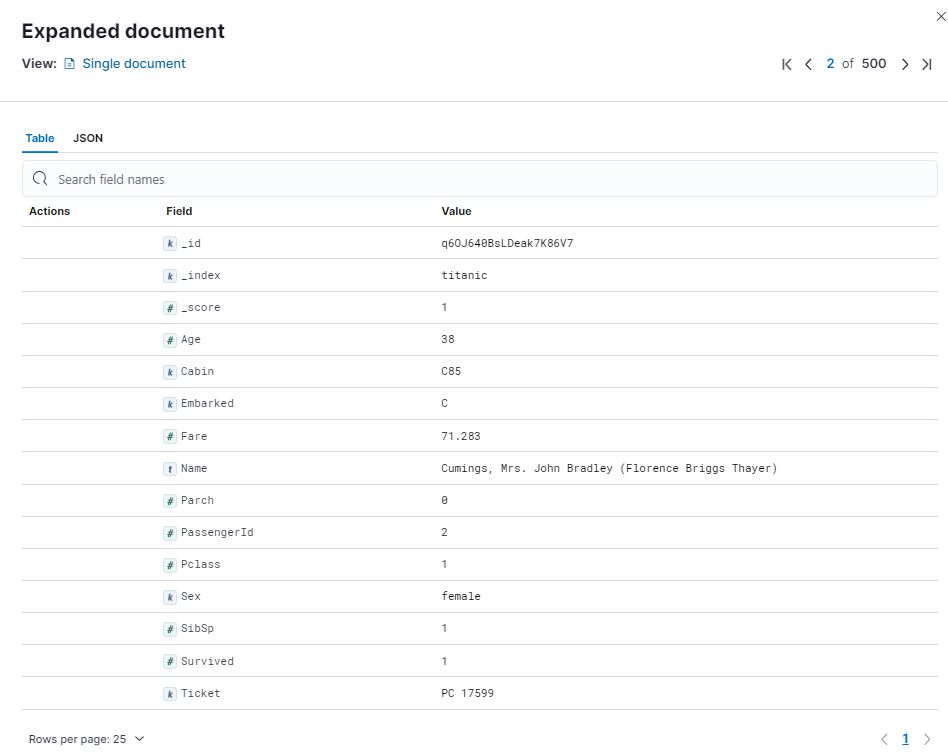
\includegraphics[width=1\linewidth]{img/kibana6.png}
    \caption{Visualización de un registro en concreto.}
    \label{fig:kibana6}
\end{figure}

Un apartado que resulta interesante de la funcionalidad \textit{Discover} es el de \textit{Field statistics} (ver ilustración  \ref{fig:kibana5}), en el cuál se muestran datos estadísticos útiles y precisos de cada campo presente en el índice, como pueden ser los valores únicos o la distribución de los valores.

\begin{figure}
    \centering
    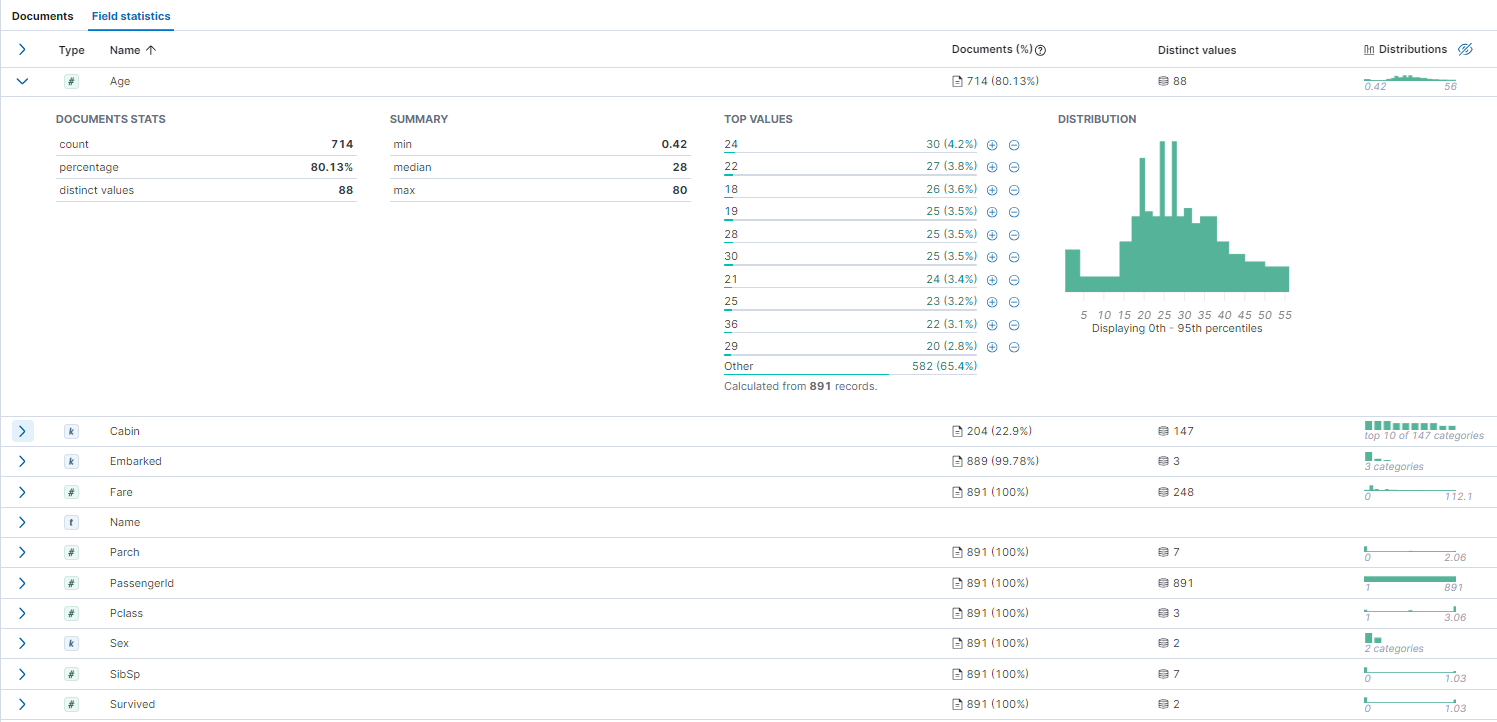
\includegraphics[width=1\linewidth]{img/kibana7.png}
    \caption{Visualización de \textit{Field Statistics}.}
    \label{fig:kibana5}
\end{figure}

\paragraph{}
\paragraph{}

Cuando se tiene comprendido la funcionalidad \textit{Discover}, se puede pasar a la parte más interesante, que es la funcionalidad \textit{Dashboards} (ver ilustración  \ref{fig:kibana8}) , en la cuál se realiza la parte más visual e intuitiva de todo el sistema ELK.

\begin{figure}
    \centering
    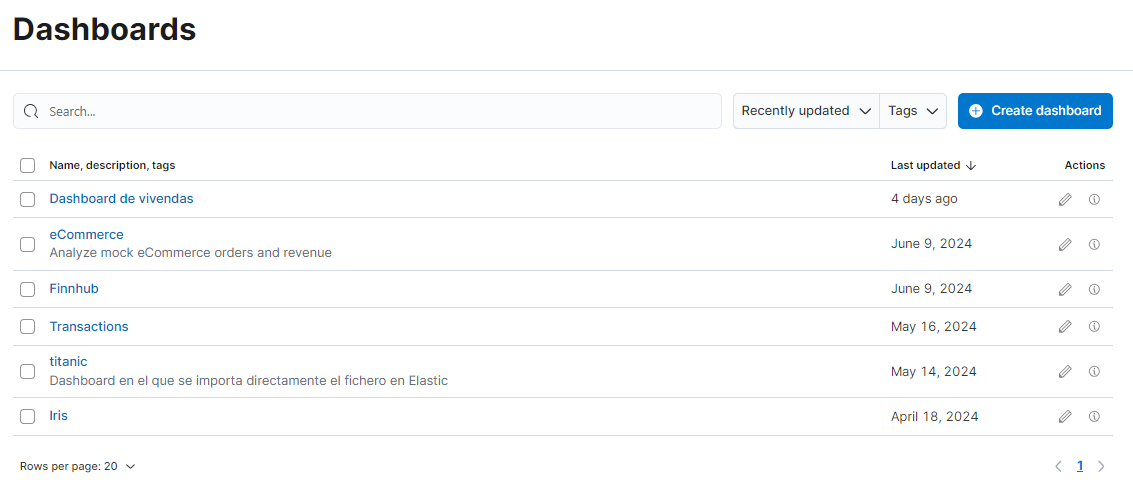
\includegraphics[width=1\linewidth]{img/kibana8.png}
    \caption{Visualización inicial de la funcionalidad \textit{Dashboards}.}
    \label{fig:kibana8}
\end{figure}

En esta sección, al igual que en la anterior, se va a explicar en el \textit{dashboard} proveniente del índice \textit{titanic}, equivalente al primero de los escenarios tratados.
La primera función a destacar es la de la posibilidad de filtrar los campos en función de los valores que se quieran (ver ilustración  \ref{fig:kibana9}). Los filtros se añaden desde la opción \textit{Controls}, pudiendo elegir si el filtro va a ser temporal o en función de los campos presentes. En este ejemplo se ha establecido un filtrado en función de la edad del pasajero (ver ilustración  \ref{fig:kibana10}), pudiendo configurar la etiqueta mostrada, el campo sobre el que se aplica el filtro o el tamaño que tendrá en el \textit{dashboard}.

\begin{figure}
    \centering
    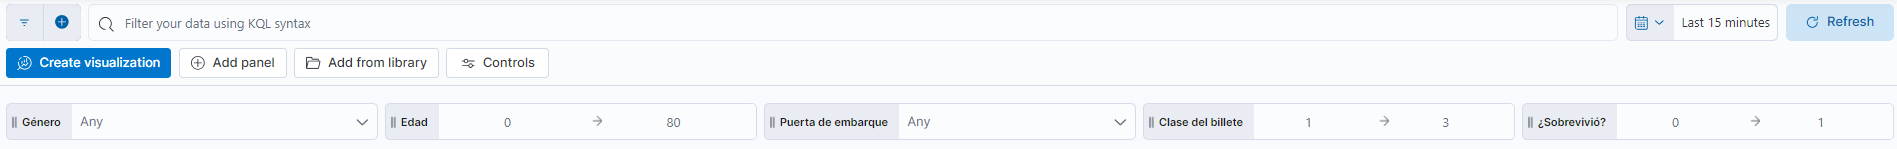
\includegraphics[width=1\linewidth]{img/kibana9.png}
    \caption{Apartado de filtrado del \textit{dashboard}.}
    \label{fig:kibana9}
\end{figure}

\begin{figure}
    \centering
    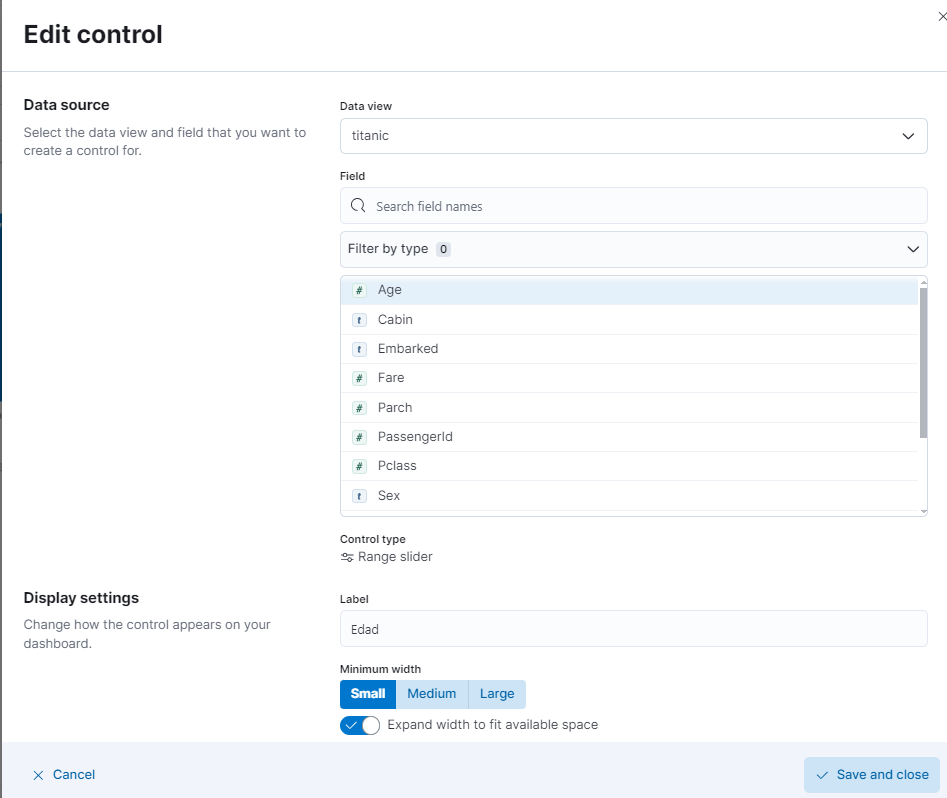
\includegraphics[width=1\linewidth]{img/kibana10.png}
    \caption{Edición de un filtro del \textit{dashboard}.}
    \label{fig:kibana10}
\end{figure}

Antes de entrar en las visualizaciones, se quiere destacar la opción de permitir añadir un panel con toda la información de los datos sobre los que está trabajando el \textit{dashboard}, a modo de atajo sin entrar al \textit{Discover}. Esto se puede realizar desde la opción \textit{Add Library} (ver ilustración  \ref{fig:kibana11}), especificando el índice que se quiere mostrar.

\begin{figure}
    \centering
    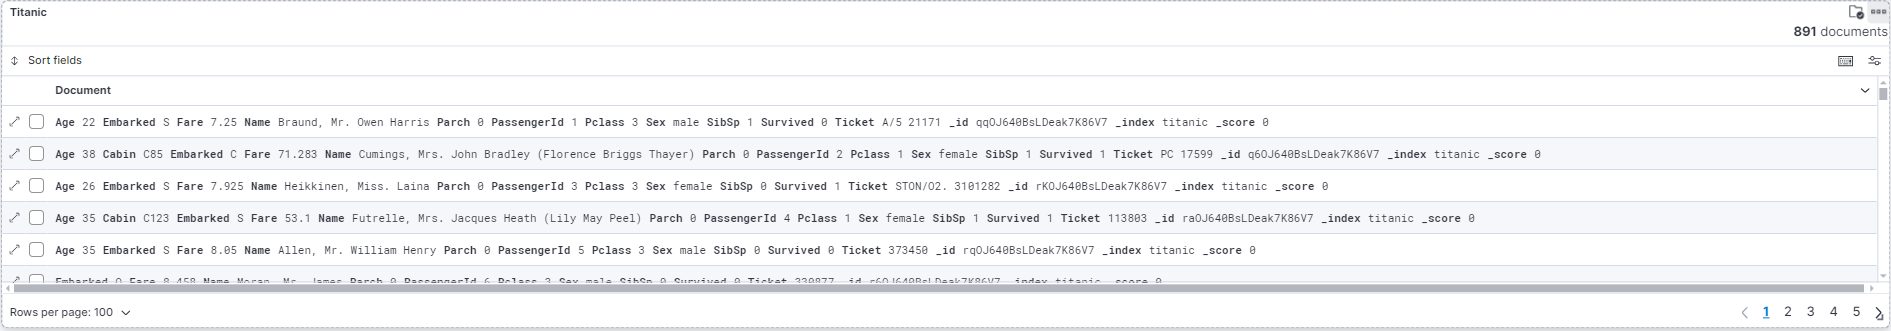
\includegraphics[width=1\linewidth]{img/kibana11.png}
    \caption{Panel mostrando los datos del índice del \textit{dashboard}.}
    \label{fig:kibana11}
\end{figure}

\paragraph{}
\paragraph{}


Habiendo explicado estas funciones secundarias que ofrece la funcionalidad \textit{Dashboards} de Kibana, es momento de exponer la función que permite crear visualizaciones con los datos del índice. Esto se realiza desde la opción \textit{Create visualization}. La visualización más sencilla es la de \textit{Metric}, en la cuál se puede especificar que se le aplique una función sencilla a un campo en concreto, en este ejemplo se ha hecho un conteo de todos los registros (ver ilustración  \ref{fig:kibana12}), y en este otro un conteo solo de los supervivientes con una fórmula usando sintaxis KQL (ver ilustración  \ref{fig:kibana13}).

\begin{figure}
    \centering
    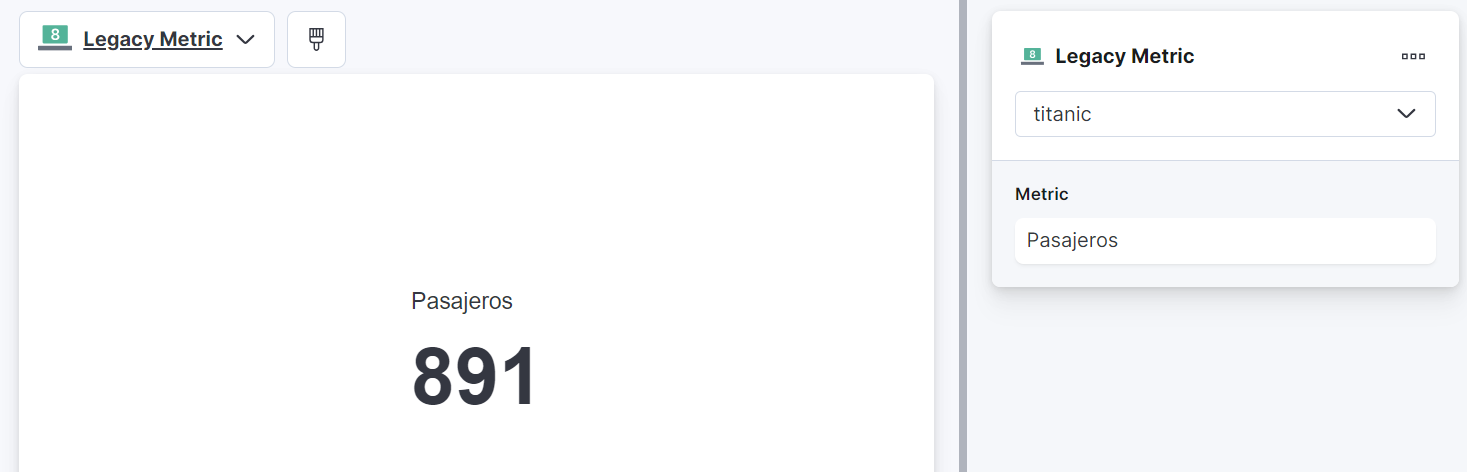
\includegraphics[width=1\linewidth]{img/kibana12.png}
    \caption{Métrica del conteo del número de parajeros.}
    \label{fig:kibana12}
\end{figure}
\begin{figure}
    \centering
    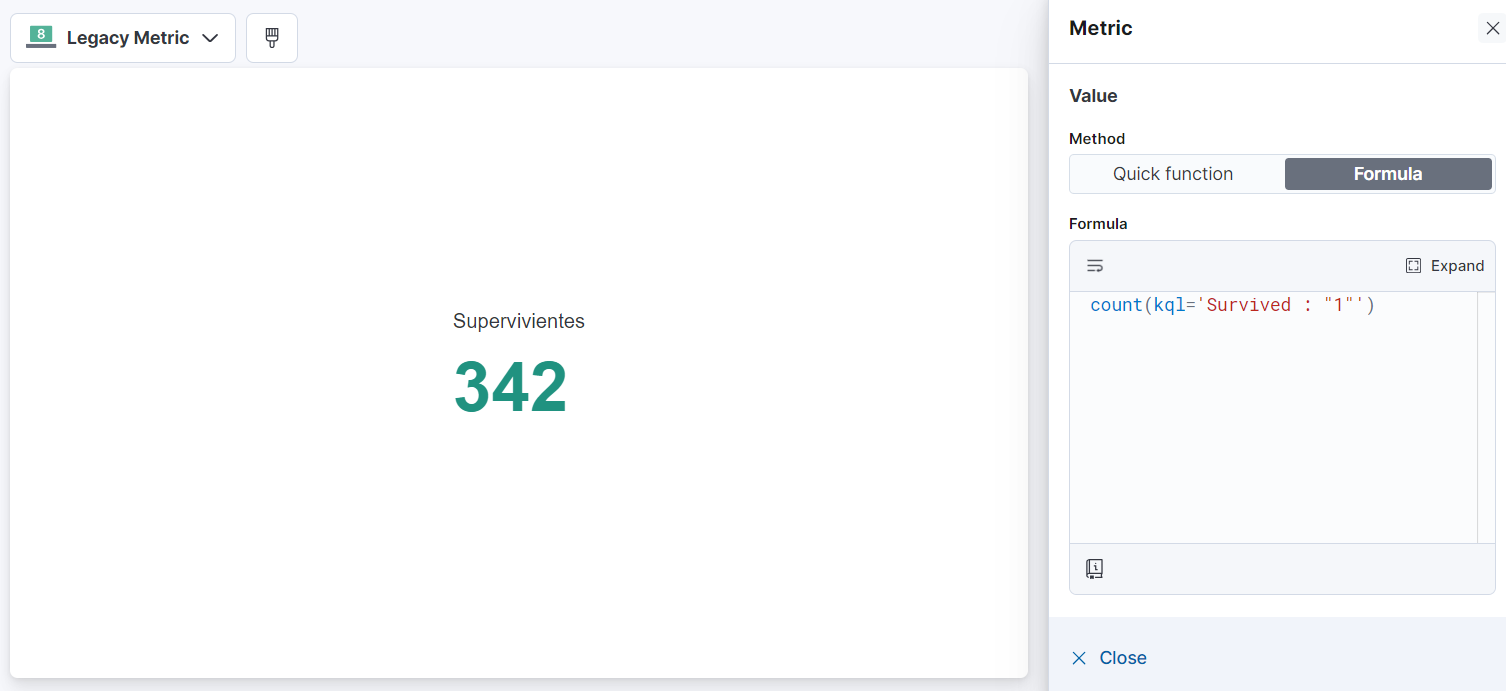
\includegraphics[width=1\linewidth]{img/kibana13.png}
    \caption{Métrica de conteo del número de supervivientes.}
    \label{fig:kibana13}
\end{figure}

Otra visualización interesante es la de los gráficos de barras, en los cuáles hay que especificar que campo se quiere usar para cada eje, y si se quiere aplicar alguna función sobre los mismos.

En este ejemplo se está realizando un conteo del número de pasajeros clasificados por género (ver ilustración  \ref{fig:kibana14}, tomando como referencia el campo \textit{Género} para el eje horizontal representando en color azul los hombres y en rosa las mujeres, y el campo \textit{Records} para el eje vertical especificando que se realize un conteo de los valores.

\begin{figure}
    \centering
    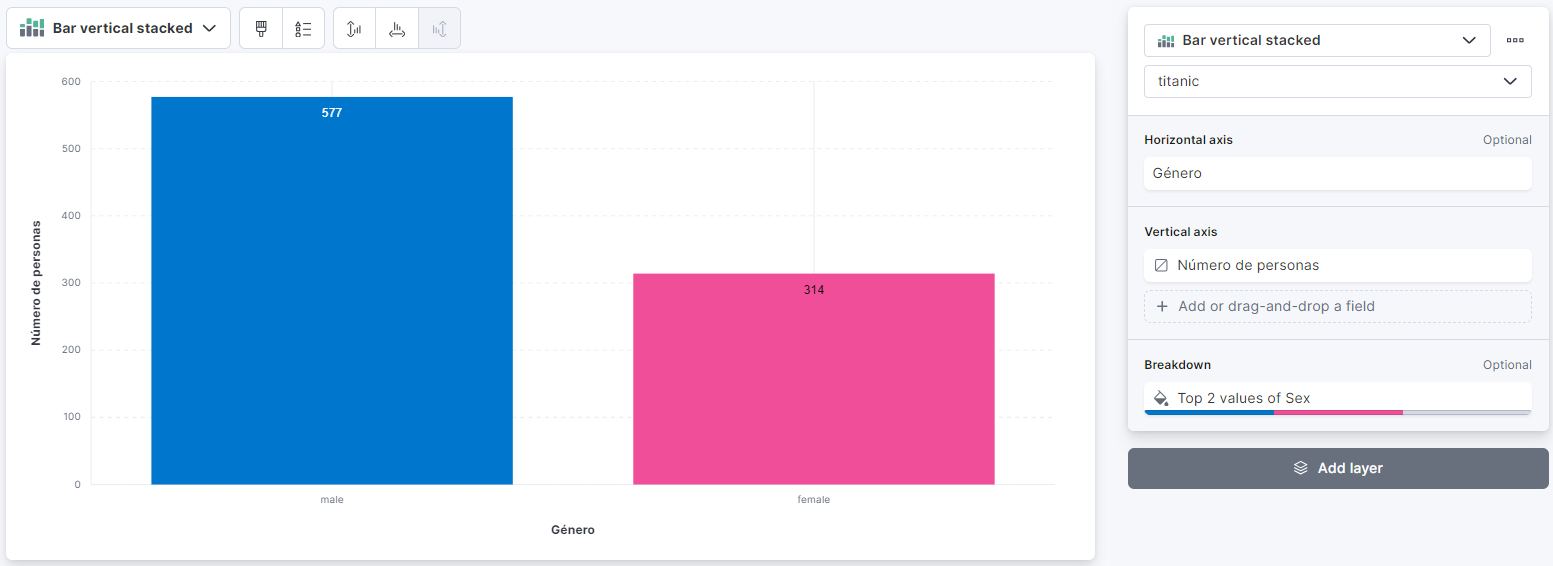
\includegraphics[width=1\linewidth]{img/kibana14.png}
    \caption{Gráfico de barras mostrando el número de pasajeros por género.}
    \label{fig:kibana14}
\end{figure}

Otro tipo de visualización que resulta intersante es la del gráfico en forma de donut, en el cuál en este ejemplo se muestra el porcentaje de pasajeros por clase de billete (ver ilustración \ref{fig:kibana15}, especificando que se va a realizar un filtrado por intervalos del campo \textit{Pclass} que es el que contiene la información pudiendo modificar las formas y colores del gráfico.

\begin{figure}
    \centering
    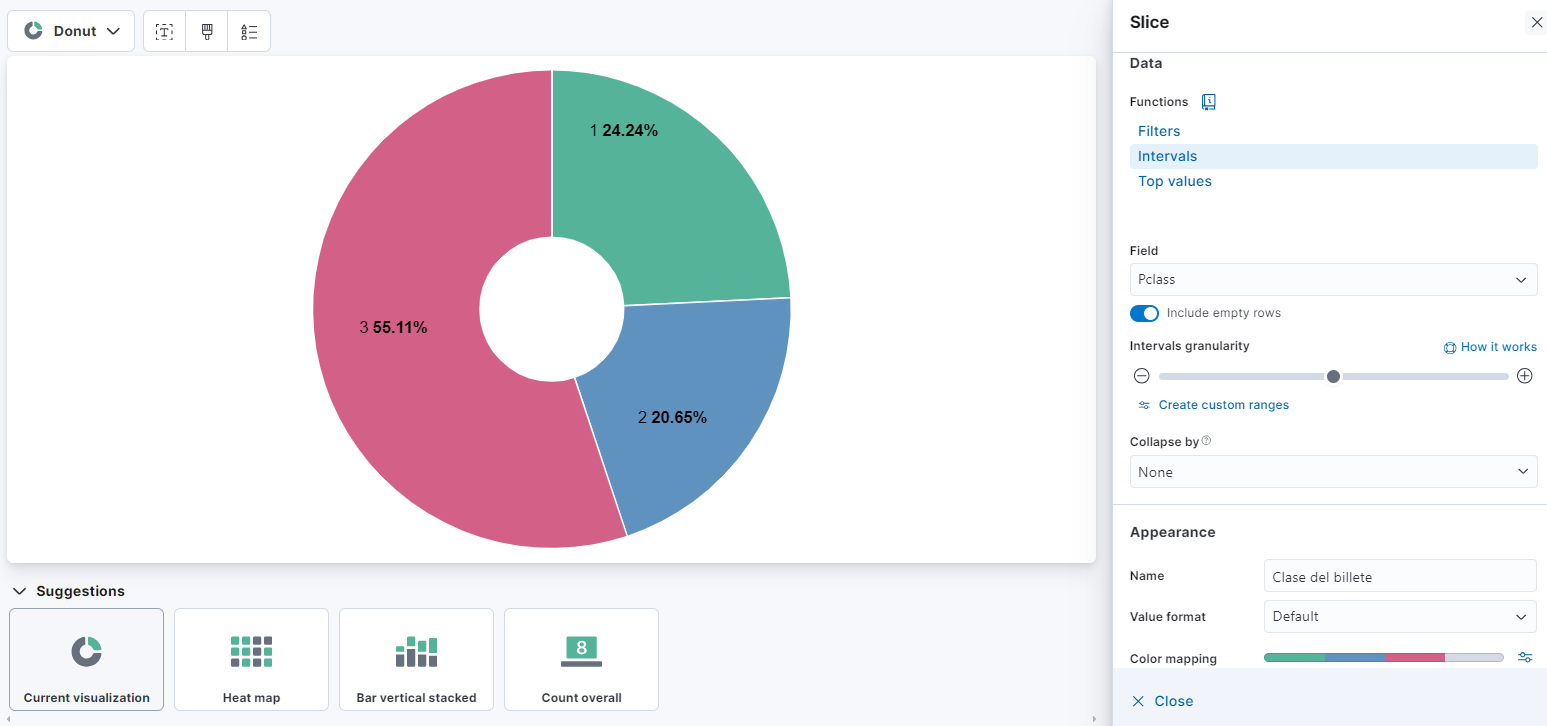
\includegraphics[width=1\linewidth]{img/kibana15.png}
    \caption{Gráfico de donut mostrando el porcentaje de pasajeros por clase de billete.}
    \label{fig:kibana15}
\end{figure}

Un gráfico presente en este \textit{dashboard} y que resulta interesante visualmente es el de un gráfico de barras apiladas (ver ilustración \ref{fig:kibana16}), en este ejemplo se muestra en el eje horizontal la edad de los pasajeros y en el eje vertical el número de pasajeros estableciendo como diferencidador para el apilamiento el género de los mismos, esto se hace desde la función \textit{Breakdown} tomando como referencia los valores del campo \textit{Sex}.

\begin{figure}
    \centering
    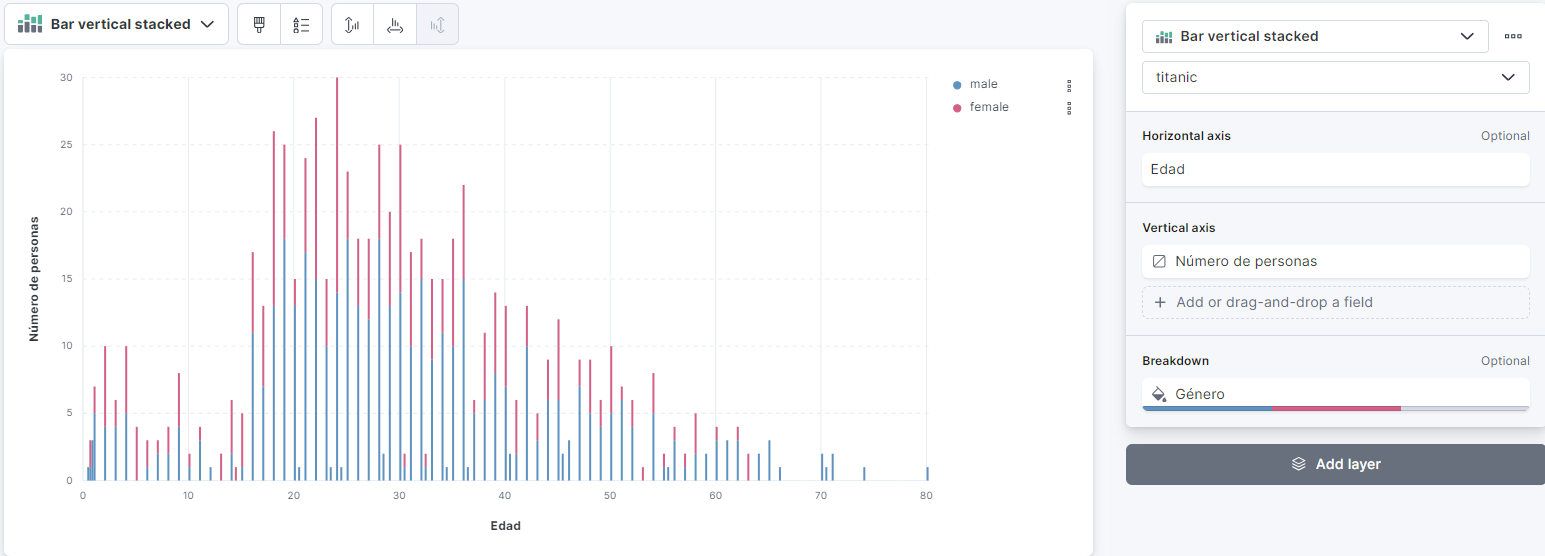
\includegraphics[width=1\linewidth]{img/kibana16.png}
    \caption{Gráfico de barras apiladas mostrando la edad del número de pasajeros en función del género.}
    \label{fig:kibana16}
\end{figure}

Además de las visualizaciones mencionadas, Kibana ofrece visualizaciones similares en forma gráficos de barra horizontales, gráficos de area, mapas de calor o mosaicos. También incluye paneles más avanzados que requieren de datos más detallados como pueden ser mapas o streams de un log (ver ilustración  \ref{fig:kibana17}, en este \textit{dashboard} de la \href{https://www.elastic.co/es/blog/kibana-3-0-0-ga-now-available}{página oficial} de Kibana se pueden observar algunos de estos paneles (ver ilustración  \ref{fig:kibana18}.

\begin{figure}
    \centering
    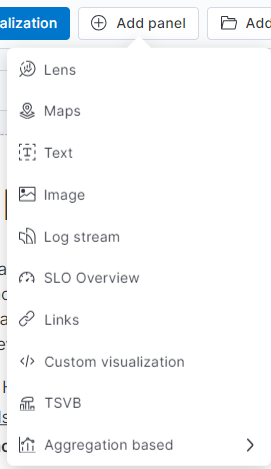
\includegraphics[width=1\linewidth]{img/kibana17.png}
    \caption{Paneles más avanzados que ofrece Kibana.}
    \label{fig:kibana17}
\end{figure}

\begin{figure}
    \centering
    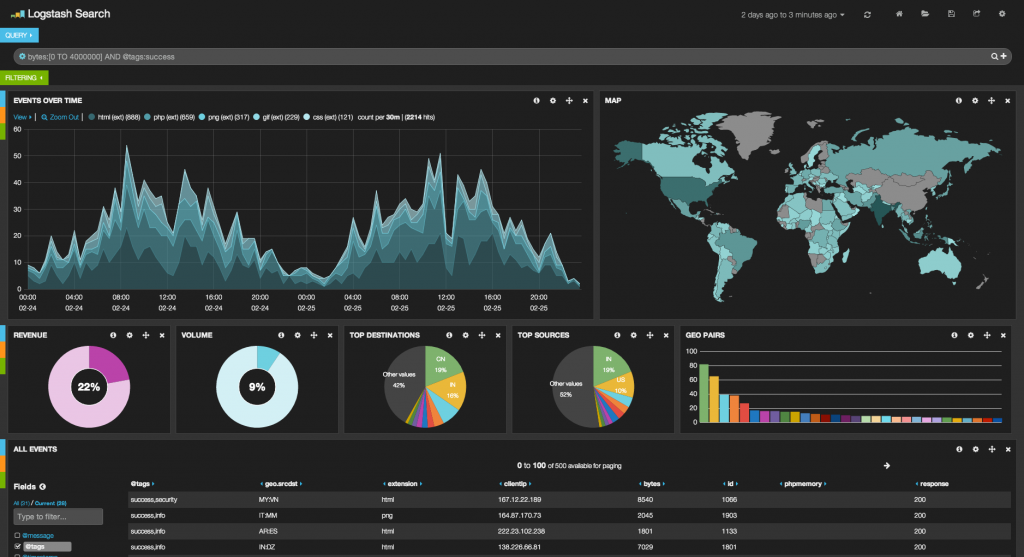
\includegraphics[width=1\linewidth]{img/kibana18.png}
    \caption{\textit{Dashboard} con paneles avanzados de Kibana.}
    \label{fig:kibana18}
\end{figure}

\paragraph{}
\paragraph{}


Una vez se da por finalizado la adición de visualizaciones y paneles al gráfico, este se puede guardar en el estado actual para poder ser modificado o exportado posteriormente desde la opción \textit{Save} en la esquina superior derecha. También se incluye una opción para visualizar el \textit{dashboard} como si se fuera un espectador desde \textit{Switch to view mode} (ver ilustración \ref{fig:kibana19}, permitiéndo comprobar que todo está correcto.

\begin{figure}
    \centering
    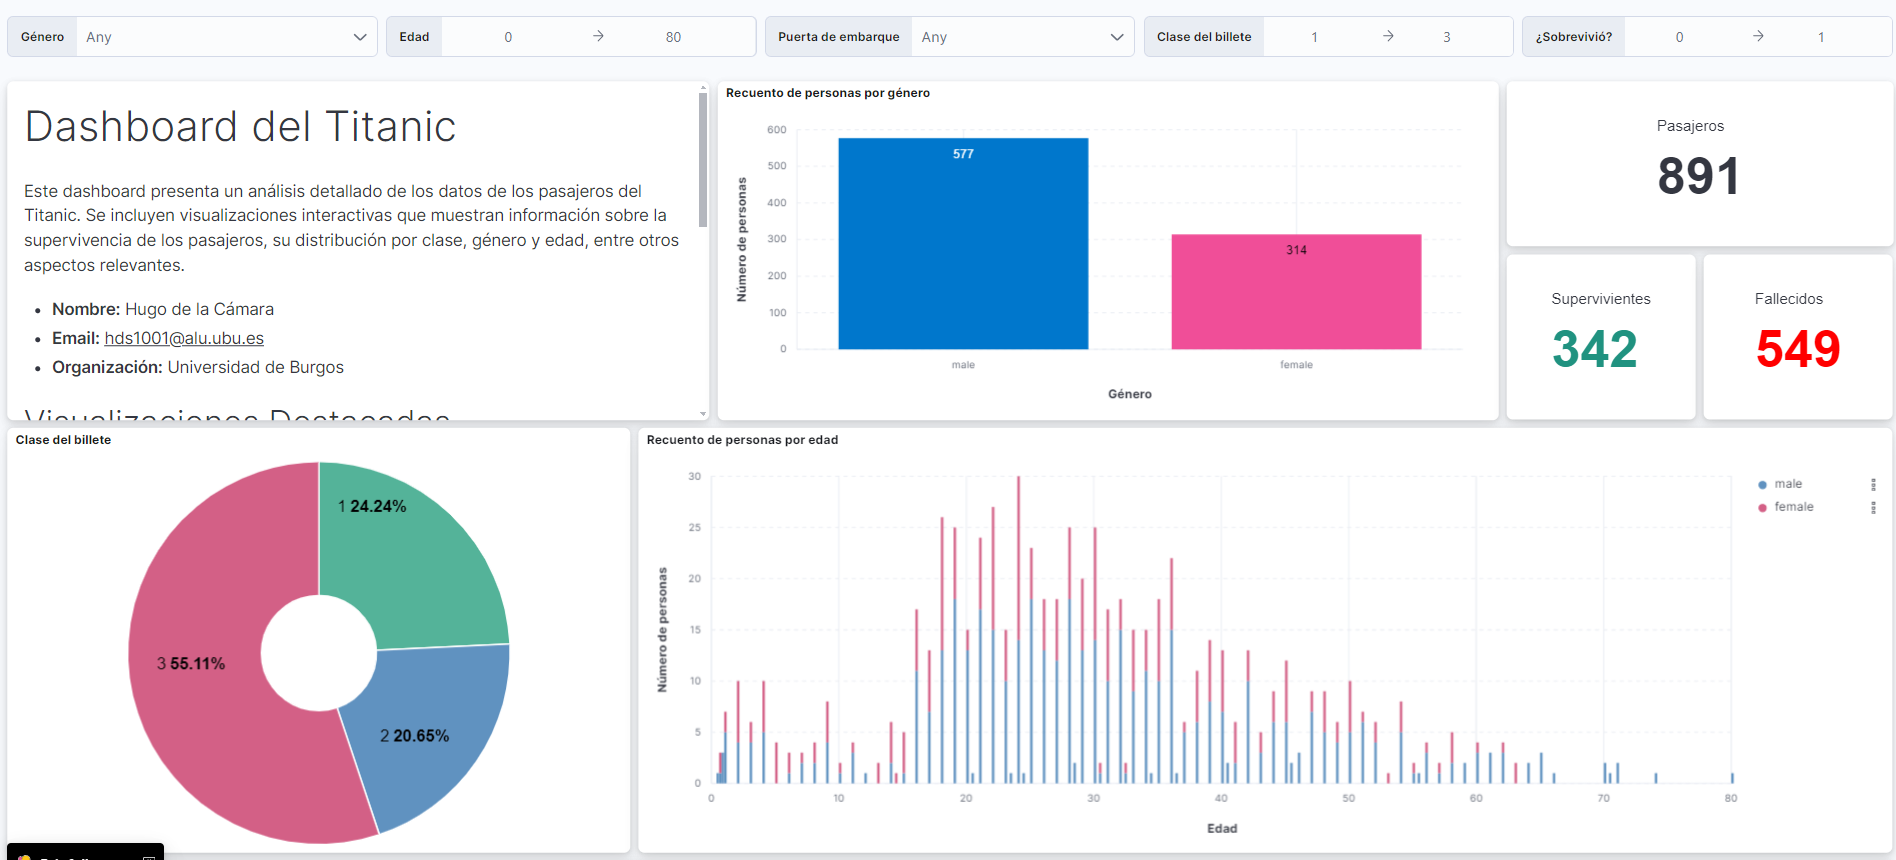
\includegraphics[width=1\linewidth]{img/kibana19.png}
    \caption{Visualización general del \textit{dashboard} desde el modo espectador de Kibana.}
    \label{fig:kibana19}
\end{figure}
